\documentclass{article}
\usepackage{graphicx}
\usepackage{float}
\usepackage{amsmath}
\usepackage{amsfonts}
\usepackage{amssymb}
\usepackage{hyperref}
\usepackage{esint}
\usepackage[utf8]{inputenc}
\usepackage[a4paper, portrait, margin=0.75in]{geometry}
\setlength\parindent{0pt}
\usepackage[italian]{babel}
\usepackage{tikz}
\usepackage{circuitikz}





\hypersetup{
    colorlinks=true,
    linkcolor=black,
    filecolor=magenta,
    urlcolor=blue,
    pdftitle={Tecnologie internet},
    pdfpagemode=FullScreen,
}


\begin{document}
    \author{kanopo}
    \title{APPLICAZIONI INDUSTRIALI ELETTRICHE ED ELETTRONICA (MODULO 1)}
    \date{2022}

    \maketitle
    \tableofcontents

    \listoffigures
    \listoftables

\section{Elementi di economia d'impresa}

ho perso il riassunto da pag 0 a pag 55
dio cane
\section{Introduzione alla gestione aziendale}
\subsection{Gestione d'impresa e attività decisionale}


\begin{itemize}
    \item L'impresa è un sistema socio tecnico aperto
    \item gli obiettivi vengono perseguiti con l'attività decisionale(migliorare produzione e soddisfazione cliente)
\end{itemize}

\begin{figure}[H]
    \centering
    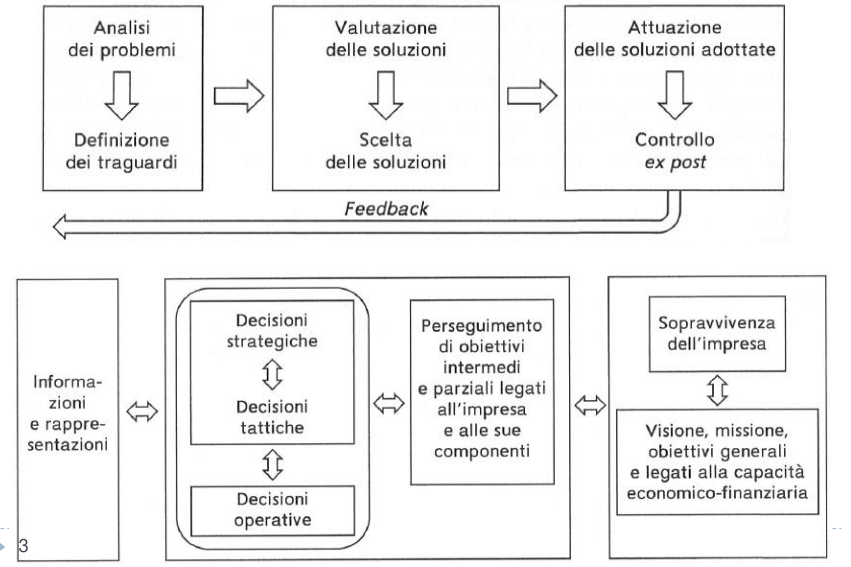
\includegraphics[width=0.7\linewidth]{1/img/Screenshot from 2022-07-03 11-30-16.png}
\end{figure}

\subsection{Criteri di scelta nelle decisioni d'impresa}


3 criteri:
\begin{itemize}
    \item efficacia: scelta e realizzazione degli obbiettivi
    \item efficienza: minimizzare le risorse
        \begin{itemize}
            \item produttività: effcienza tecnica
            \item economicità: effcienza economica
        \end{itemize}
    \item redditività
\end{itemize}

\begin{figure}[H]
    \centering
    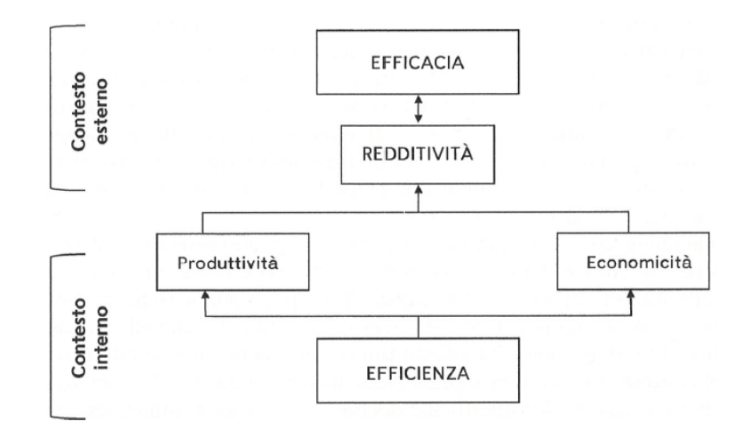
\includegraphics[width=0.5\linewidth]{1/img/Screenshot from 2022-07-03 11-35-16.png}
\end{figure}

\subsection{Incertezza e ambiguità nelle decisioni d'impresa}

\begin{figure}[H]
    \centering
    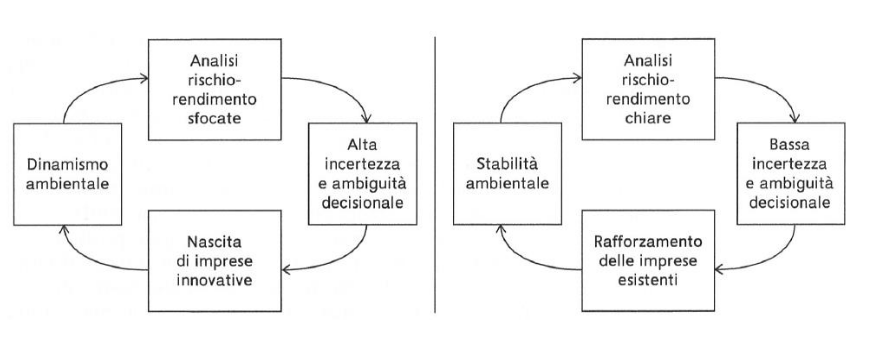
\includegraphics[width=0.7\linewidth]{1/img/Screenshot from 2022-07-03 11-36-56.png}
\end{figure}

\subsection{Le aree funzionali di gestione}

\begin{figure}[H]
    \centering
    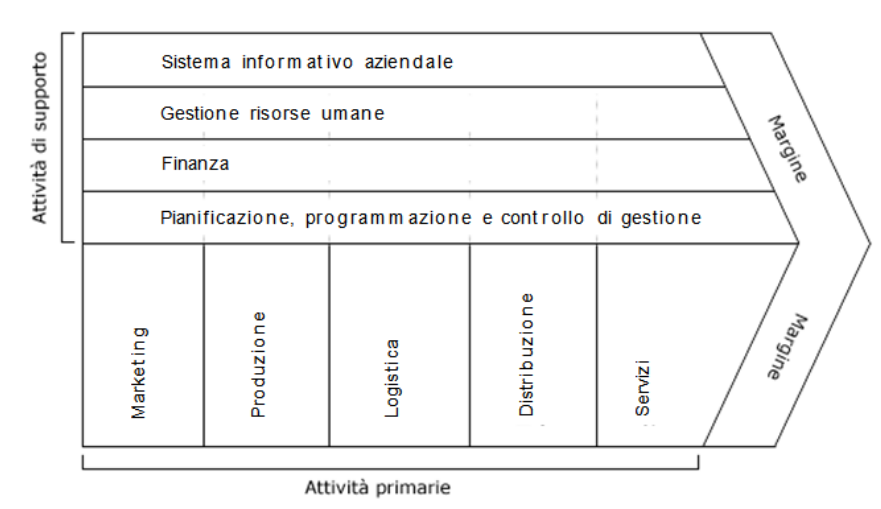
\includegraphics[width=0.7\linewidth]{1/img/Screenshot from 2022-07-03 16-14-51.png}
\end{figure}

\subsection{Marketing}
Attività volte a soddisfare le esigenze dei consumatori fornendo prodotti e servizi.

\subsection{Produzione}
Attività volte alla realizzazione di un prodotto o servizio.

Segue breve classificazione di processi produttivi:
\begin{figure}[H]
    \centering
    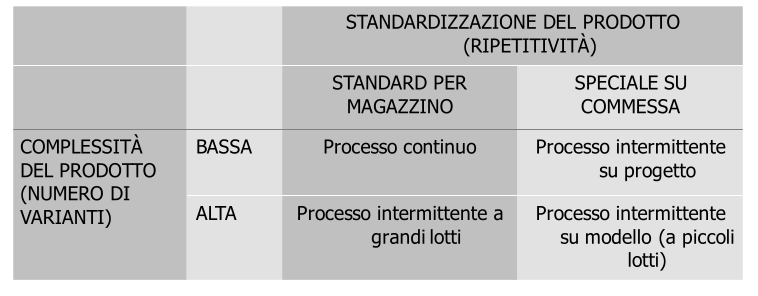
\includegraphics[width=0.5\linewidth]{1/img/Screenshot from 2022-07-04 14-59-14.png}
\end{figure}


La valutazione dell'investimento industriale richiede di considerare i seguenti aspetti:
\begin{itemize}
    \item domanda del mercato
    \item scelte strategiche relative al decentramento produttivo(aka far fare le cose a una schiaffo/ora e sfruttare i bambini)
    \item localizzazione impianti e magazzini
    \item organizzazioen del lavora nello stabilimento
    \item obsolescenza tecnologica del prodotto e dell'impianto
\end{itemize}

\subsection{Logistica}
Attività per la gestione del flusso di beni dal fornitore, all'impresa e al cliente.


La distribuzione finale al cliente ha varie tipologie:
\begin{itemize}
    \item distribuzione selettiva(pochi intermediari)
    \item distribuzione esclusiva(unico distributore autorizzato)
    \item distribuzione intensiva(più punti vendità possibile)
\end{itemize}

\subsection{Sistema informativo aziendale}

Tipo la business intelligence in big data e business intelligence, raccoglie, conserva ed elabora dati per migliorare il processo decisionale.


\begin{itemize}
    \item EDP (Electronic Data Processing, sistema di
    elaborazione dati)

    \item MIS (Management Information System, sistema di
    gestione delle informazioni)

    \item DSS (Decision Support Sistem, sistema di supporto alle
    decisioni)
\end{itemize}


\subsection{Finanza}

Attività volta a reperire capitali finanziari e ad utilizzarli correttamente con la programmazione dell'attviità d'impresa.

Raggiungimento di tre equilibri:
\begin{itemize}
    \item redditività(equilibrio ricavi costi)
    \item solvibilità(equilibrio fonti impieghi)
    \item liquidità(equilibrio entrate e uscite)
\end{itemize}


Questo campo include attività come la gestione finanziaria in caso di fallimento, scelta degli investimenti e analisi di bilancio.


\subsection{Pianificazione strategica, programmazione e controllo di gestione}
\begin{itemize}
    \item pianificazione e programmazione: si completano con il controllo di gestione
    \item controllo di gestione: indici di rendimento e poi controllo direzzionale
    \item controllo direzionale: controllo operativo, economico-finanzioario e controllo strategico
    \item controllo operativo: check periodico della performance
    \item controllo economico finanziario: previsionale e storico
\end{itemize}

\begin{figure}[H]
    \centering
    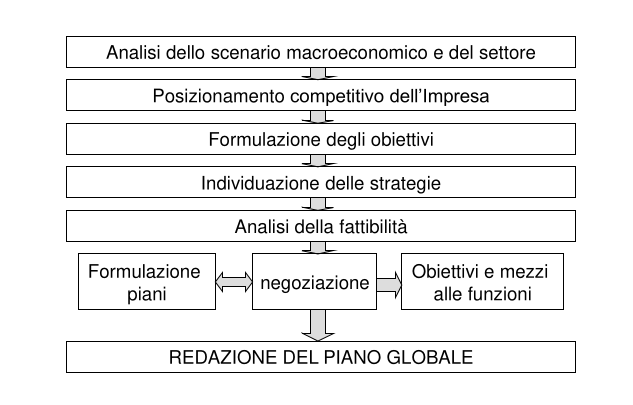
\includegraphics[width=0.5\linewidth]{1/img/Screenshot from 2022-07-04 17-21-38.png}
\end{figure}

\begin{figure}[H]
    \centering
    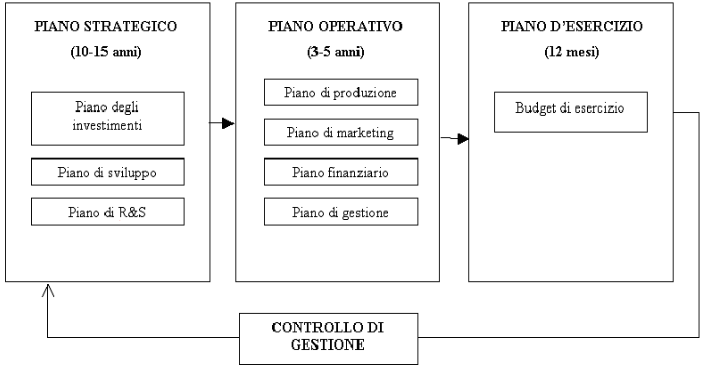
\includegraphics[width=0.5\linewidth]{1/img/Screenshot from 2022-07-04 17-22-15.png}
\end{figure}


\subsection{Gestione delle risorse umane}
Composta da gestione del personale e dall'organizzazione del personale.

L'organizzazione include la definizione di ruoli per il personale e l'assetto organizzativo in generale.


L'aspetto gestionale:
\begin{itemize}
    \item riperimento del personale
    \item selezione
    \item addestramento
    \item altre menate
\end{itemize}


    
\end{document}